\documentclass[anon=true]{ceurart}

\sloppy

\usepackage{paralist}
\usepackage{todonotes}
\usepackage{caption, subcaption} %% for subfigures, subfig is outdated
\usepackage{stmaryrd}

%\usepackage{amsmath}
%\usepackage{amssymb}

\usepackage{adjustbox}
\usepackage{listings}
\presetkeys{todonotes}{color=red!40,size=\tiny}{}
\setlength{\marginparwidth}{2.5cm}
\usepackage{xspace}



\newcommand{\NAME}{RAW-JENA\xspace}
\newcommand{\TODO}[1]{\textcolor{red}{#1}}
\newcommand{\REF}[0]{\textcolor{purple}{REF}\xspace}
\newcommand{\WANDER}{Wander~Join\xspace} %% two separated words, maybe should textsc{}

\copyrightyear{2023}
\copyrightclause{Copyright for this paper by its authors.
  Use permitted under Creative Commons License Attribution 4.0
  International (CC BY 4.0).}

\conference{ISWC'23: International Semantic Web Conference,
  November 06--10, 2023, Athens, Greece}

\title{\NAME: Approximate Query Processing\\for SPARQL Endpoints}

%% \author[1]{Julien Aimonier-Davat}[%
%%   orcid=0000-0001-6707-0204,
%%   email=name@example.com,
%% ]

%% \author[1]{Minh-Hoang Dang}[%
%%   % orcid=,
%%   email=name@example.com,
%% ]

%% \author[1]{Pascal Molli}[%
%%   orcid=0000-0001-8048-273X,
%% ]

%% \author[1]{Brice N{\'e}delec}[%  
%% ]

%% \author[1]{Hala Skaf-Molli}[%
%%   orcid=0000-0003-1062-6659,
%% ]

\author[1]{Author one}[%
]

\author[1]{Author two}[%
]

% \address[1]{Nantes Universit{\'e}, CNRS, LS2N, UMR 6004, F-44000 Nantes, France}
\address[1]{Institution and address}



\begin{document}

\maketitle


\begin{abstract}
  Sampling-based approximate query processing (S-AQP) has many
  important use-cases in RDF including computing large scale
  statistics, embeddings, join orderings, approximate aggregations,
  summaries, exploratory queries. However, current SPARQL endpoints
  have no support for S-AQP, and many queries just time-out on public
  SPARQL endpoints. In this demonstration, we present \NAME: an
  extension of Apache Jena to support S-AQP for conjunctive SPARQL
  queries relying on random walks. \NAME delivers partial random
  results along with cardinality estimates in a pay-as-you-go fashion
  with a logarithmic time complexity.
\end{abstract}

\begin{keywords}
  SPARQL \sep
  Sampling \sep
  Approximate query processing \sep
  Random walks
\end{keywords}


%
\section{Introduction}

Sampling-based approximate query processing (S-AQP)
~\cite{DBLP:conf/sigmod/AgarwalMKTJMMS14} drastically reduce query
execution time to deliver approximated results with error
estimation. S-AQP has many important use-cases in RDF including
computing large scale
statistics\cite{soulet2019anytime,10.1007/978-3-319-18818-8_14},
computing embeddings with random walks\cite{ristoski2016rdf2vec}, join
orderings for query optimisation\cite{DBLP:conf/cidr/LeisRGK017},
approximated
aggregations~\cite{DBLP:journals/tods/LiWYZ19,DBLP:conf/cikm/00010XYPZ2},
summaries computation~\cite{10.1007/978-3-030-49461-2_10}, exploratory
queries~\cite{DBLP:conf/sigmod/AgarwalMKTJMMS14}.  However, given a
query, current SPARQL endpoints have no support for approximated query
processing. This is a major issue, especially  for public SPARQL endpoints where
many queries just time-out without S-AQP support. To illustrate, suppose you just want to draw a
random triple from Wikidata as proposed in~\cite{soulet2019anytime} with query $Q_s$:
%
\verb+select * {?s ?p ?o} LIMIT 1 OFFSET r+
%
where $r$ is a random number between 0 and the cardinality of Wikidata
 ie. $0<r<12B$. Unfortunately when $r>100M$,
$Q_s$ time-out  returning no result\footnote{other methods
  to sample relying on ORDER BY rand() also time-out}. Some SPARQL endpoints
  providers provides ad-hoc solutions to compute more efficiently
  random triples from triple
  patterns\footnote{\url{https://docs.stardog.com/query-stardog/sampling-service\#sampling-service.}},
  b,
  ~\footnote{\url{https://docs.openlinksw.com/virtuoso/rndsalltr/}}. However,
   the sampling is
  limited to triple patterns and the underlying complexity is not
  established. On SPARQL, there is nothing equivalent to the
  TABLESAMPLE clause that is part of the SQL standard since 2003.

% From the state of art~\cite{DBLP:conf/cidr/LeisRGK017}, we know that
% is possible to draw a random triple from a triple pattern in
% logarithmic time using the internal index of a TripleStore. Extending
% to BGP support just multiply this complexity by the number of triple
% pattern in the query. Sampling queries makes sense only if the
% approximation error can also be estimated ie. for a query

  In this demonstration, we extended JENA to support efficiently
  S-AQP for core conjunctive
  SPARQL queries.  Given a SPARQL $Q$ query and a budget in time,
  \NAME~\footnote{\url{https://github.com/Chat-Wane/raw-jena}} is able
  to deliver random results along with a cardinality estimation of the
  total number of results. Our approach relies on random
 walks as defined in WanderJoin\cite{li2016wanderjoin}. This approach
 has been proven accurate on the G-Care
 benchmark\cite{DBLP:conf/sigmod/ParkKBKHH20} for RDF datasets. Thanks
 to traditional indexing schema of RDF \footnote{SPO,POS,OSP}, random
 walks for conjunctive queries can be executed in $k.log(|G|)$ where
 $k$ is the number of triple patterns in the query and $|G|$ the size
 of the dataset. Thanks to the random walk approach, \NAME converges
 to complete results ie. sampling the query multiple times returns
  more result and improve the accuracy of the cardinality.
  %

  For the demonstration, we uploaded the Wikidata
  Benchmark\cite{angles2022wdbench} in \NAME. As many queries are
  timing-out on WDbench, users can see what they can obtain with the
  same queries processed with S-AQP and how results and
  accuracy evolve with the pay as you go approach.

  The overall objective of the demonstration is to show the usefulness
  of S-AQP for SPARQL endpoints, the feasability of implementation on
  well-known engine, and how the eco-system of public sparql endpoints
  can take advantage of such new processing regime.






% \section{Introduction (from quota)}

% Public SPARQL endpoints as Wikidata or DBPedia allow anyone to execute
% any SPARQL queries. However, due to fair use policies of public SPARQL
% endpoints, there is no guarantee of termination with complete
% results. On Wikidata, queries are stopped after 60s returning partial
% results~\footnote{\url{https://www.mediawiki.org/wiki/Wikidata_Query_Service/User_Manual}},
% On Dbpedia, the maximum execution time is set to 120 second with a
% maximum 10000
% results~\footnote{\url{https://www.dbpedia.org/resources/sparql/\#ratesandlimits}}. Consequently,
% it exist a class of SPARQL queries that time-out when executed on
% public SPARQL endpoint~\cite{DBLP:conf/semweb/MalyshevKGGB18} that is
% the base for the Wikidata benchmark\cite{angles2022wdbench}.

% It is impossible for a SPARQL endpoint to ensure that any query
% returns complete results in fixed time. However, it is possible to
% ensure to return a sample of results in fixed time, along with an
% estimation of the cardinalities of complete results. For example, the
% $Q_1$ of figure~\ref{fig:q1-nojo} timeout on Wikidata, returning
% partial non-random results. However, it is possible to sample the
% evaluation of Q1, returning random results along with an estimation of
% the cardinality of results with a confidence interval. For a budget of
% 1s, on JENA-RAW, we obtained 50 results on potentially 1000 results
% more or less 50.

% Sampled results can be incrementally improved following a
% pay-as-go approach ie. resending the same
% query for another budget of 1s allows to get other random results with
% possible duplicates, but with an higher accuracy on cardinality.



% \begin{figure}[t]
%  \begin{center}
%   \subfloat [Query $Q_1^{J_1}$ time-out >60s] {\label{fig:q1-nojo}
%    \adjustbox{valign=T}{
%     \resizebox{0.45\textwidth}{!}{
%      \lstinputlisting[basicstyle=\scriptsize\sffamily,
%      language=sparql,numbers=none,columns=fixed,
%      showstringspaces=false]{./figures/q1w.rq}}}}
%   \subfloat [Query $Q_1^{J_2}$ forced join order $\sim 451ms$] {\label{fig:q1j2}
%    \adjustbox{valign=T}{
%     \resizebox{0.45\textwidth}{!}{
%      \lstinputlisting[basicstyle=\scriptsize\sffamily,
%      language=sparql,numbers=none,columns=fixed,
%      showstringspaces=false]{./figures/q1w-jo.rq}}}}
%  \end{center}
%  \caption{The query $Q_1$ searches for creative works and the list of
%   fiction works that inspired them. $Q_1$ time-out on
%   the Wikidata online server (>60s)}
%  \label{fig:q1}
% \end{figure}

% Sampling query evaluation has many practical use-cases that is
% currently limited as computing
% large scale statistics\cite{soulet2019anytime}, embeddings with random
% walks\cite{ristoski2016rdf2vec}, join
% orderings\cite{DBLP:conf/cidr/LeisRGK017}, approximated
% aggregations\cite{DBLP:journals/tods/LiWYZ19}.




% To validate our
% approach, we extended JENA with a sampling interface and show what can
% be obtained with fixed time for queries that traditionaly time-out on
% public endpoints.




% Random walks are important but do not have efficient implementations,
% or unsufficient API. More importantly, they are precluded to servers
% and they do not let outsiders use them.

% Could go for triple/quad patterns and it would be enough. But the more
% we push to server the more efficient.

% Especially relevant for SPARQL since we often have all indexes.

% We limit ourself to a subset of SPARQL for now. We do not process
% property paths although it would be possible. Optionals, set minus, are
% difficult.

% \todo{MUST shoot a short video to showcase \NAME. And link it.}

% Random walks enable few use-cases (from most easy to most demanding)
% such as:
% \begin{asparadesc}
% \item [Summaries] needs random walk values.
% \item [pyRDF2Vec~\cite{steenwinckel2023pyrdf2vec}] needs random walk values.
% \item [FedUP] needs the graphs of random walks.
% \item [Join ordering~\REF] needs cardinalities of random walks.
% \item [Sparklis~\cite{ferre2017sparklis}] needs random walks (at
%   least) and cardinality (optional).
% \item [Wander Join~\cite{li2016wanderjoin}] needs the cardinality of
%   random walks, failed and succeeded.
% \end{asparadesc}

%%% Local Variables:
%%% mode: latex
%%% TeX-master: "../paper.tex"
%%% End:


\section{Introduction}

Public SPARQL endpoints cannot fully execute many SPARQL queries due
to their quotas and fair-use policies. After 60 seconds, they stop
their execution and return only partial results, forbidding many use
cases such as building summaries or computing large-scale statistics.
This constitutes a major issue for building decentralized ecosystems
of public SPARQL endpoints.

Sampling-based Approximate Query Processing
(S-AQP)~\cite{DBLP:conf/sigmod/AgarwalMKTJMMS14} tackles this issue
for use cases such as computing large-scale
statistics~\cite{soulet2019anytime,10.1007/978-3-319-18818-8_14},
knowledge graph embeddings~\cite{ristoski2016rdf2vec}, join
orders~\cite{DBLP:conf/cidr/LeisRGK017}, approximate
aggregations~\cite{wang2022approximate},
summaries~\cite{10.1007/978-3-030-49461-2_10}, and exploratory
queries~\cite{DBLP:conf/sigmod/AgarwalMKTJMMS14}.  By confining query
execution to samples of large datasets, S-AQP drastically reduces
execution time, delivering approximate results with error estimates.
%
To support S-AQP in SPARQL, the evaluation of such queries \emph{must}
both
\begin{inparaenum}[(i)]
\item returns random samples, and
\item comply with fair-use policies of public SPARQL endpoints.
\end{inparaenum}
Ad-hoc methods already exist to sample knowledge graphs.  For example, a user could draw random triples from
Wikidata~\cite{soulet2019anytime} by repeatedly executing
\verb|SELECT * {?s ?p ?o} OFFSET r LIMIT 1|, where $r$ is a random
number between $0$ and the dataset size ($0<r<12B$). However, all
queries time out when $r$ is above $100M$.
%Hala: random sampling from the set of results matched by a particular SPARQL triple pattern
Some triple stores propose home-made methods for sampling triple
patterns%
\footnote{\url{https://docs.stardog.com/query-stardog/sampling-service\#sampling-service}}\textsuperscript{,}\footnote{\url{https://docs.openlinksw.com/virtuoso/rndsalltr/}},
but these solutions are limited to single triple patterns and the
underlying complexity is not established.

In this demonstration, we introduce \NAME, an extension of Apache Jena
that efficiently supports S-AQP for conjunctive SPARQL queries. \NAME
evaluates a query $Q$ over a dataset $D$ by drawing random walks
guided by $Q$, as defined in \WANDER~\cite{li2019wanderjoin}. Random
walks have two desirable properties:
\begin{inparaenum}[(i)]
\item As each random walk is \emph{independant}, a user can distribute
  its query execution into multiple requests, hence collecting and
  merging random walks in a pay-as-you-go fashion without impairing
  the fair-use policy of public SPARQL endpoints.
\item As each random walk enjoys a \emph{logarithmic time complexity},
  endpoints can draw thousands of random walks per second: the widely
  used BTree indexes of RDF stores allow endpoints to compute each
  random walk in $\mathcal{O}(|Q| \log |D|)$ where $|Q|$ is the number
  of triple/quad patterns in $Q$ and $|D|$ is the number of
  triples/quad in $D$.
\end{inparaenum}

\NAME produces random partial results instead of complete
results. Without cardinality estimates, users cannot appreciate the
quality of provided samples. In Figure~\ref{fig:raw_screenshot}, \NAME
returns $1434$ random results after $35$ seconds. By adding an
estimate of the total number of results ($26 \pm 3M$), the user
acknowledges that her sample represents but a tiny fraction of the
whole results.  Provided estimates prove highly accurate as long as
random walks remain paired with their probability of being
drawn~\cite{DBLP:conf/sigmod/ParkKBKHH20}. Despite starting from $35
\pm 15M$, \NAME improved over time, reaching $26\pm 3M$ while the
actual number of results is $25M$.

For the demonstration, we load the dump of Wikidata provided by
WDBench~\cite{angles2022wdbench} that comprises $1.2B$ triples.  We
let users choose a query among the $16$ that time out on Apache
Jena. We execute it using \NAME to highlight
\begin{inparaenum}[(i)]
\item the benefits of S-AQP for ecosystems of public SPARQL endpoints
  and
\item the feasibility of implementing S-AQP on well-known engines.
\end{inparaenum}

%% the $1.2B$ triples Wikidata dataset
%% provided by WDBench~\cite{angles2022wdbench}, and we re-execute the 16
%% queries that time out on Jena using \NAME. %S-AQP as explained in
%% Section~\ref{proposal}.
%
% Hala
%  The S-AQP results shed light on the reasons for these queries time out and provide users with valuable  information about
% Thanks to S-AQP results, users can understand
% why these queries time out. Overall, this demonstration highlights


%%% Local Variables:
%%% mode: latex
%%% TeX-master: "../paper.tex"
%%% End:


\section{\NAME}

 \begin{figure}[t]
  \begin{center}
   \subfloat [Query $Q_1^{J_1}$ time-out >60s] {\label{fig:q1-nojo}
    \adjustbox{valign=T}{
    \resizebox{0.45\textwidth}{!}{
     \lstinputlisting[basicstyle=\scriptsize\sffamily,
     language=sparql,numbers=none,columns=fixed,
     showstringspaces=false]{./figures/q1w.rq}}}}
  \subfloat [Query $Q_1^{J_2}$ forced join order $\sim 451ms$] {\label{fig:q1j2}
   \adjustbox{valign=T}{
    \resizebox{0.45\textwidth}{!}{
     \lstinputlisting[basicstyle=\scriptsize\sffamily,
     language=sparql,numbers=none,columns=fixed,
     showstringspaces=false]{./figures/q1w-jo.rq}}}}
 \end{center}
 \caption{The query $Q_1$ searches for creative works and the list of
  fiction works that inspired them. $Q_1$ time-out on
  the Wikidata online server (>60s)}
 \label{fig:q1}
\end{figure}


Pay-as-you-go \texttt{:)}.

The more the server can do, the better. But client must also be able
to process and merge incoming control information.

We enhanced Apache Jena with random walks over its default internal
storage called TDB2.



%
%% \section{Evaluation}

%% \TODO{Link to repository. Along with instructions \texttt{;)}}

%% How it improves processing time of embeddings over wikidata.

%% How it allows users to get approximate query results on wikidata
%% queries that would otherwise time out on public endpoints. 

\section{Demonstration Plan}

 \begin{figure*}
   \centering
   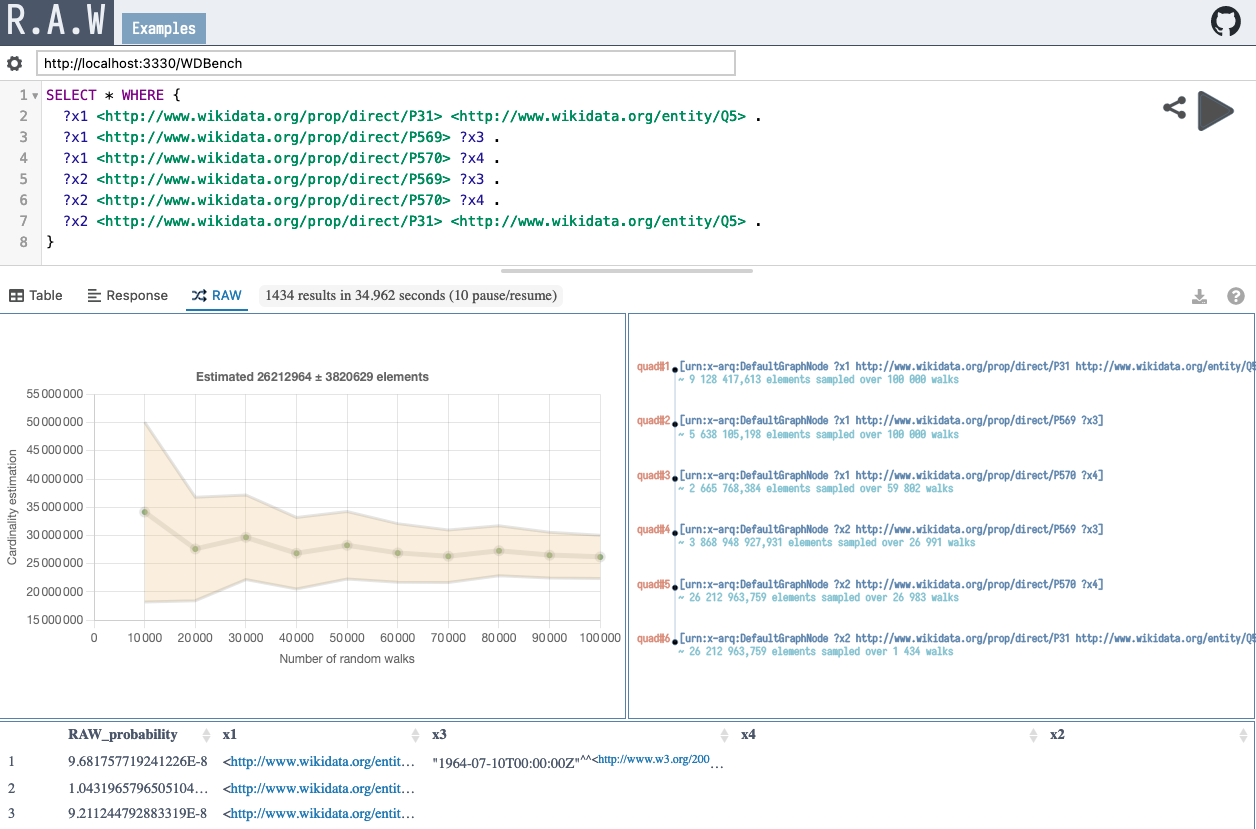
\includegraphics[width=0.85\textwidth]{figures/raw_screenshot.png}
   \caption{\label{fig:raw_screenshot}User interface of \NAME providing useful insights on the query.}
 \end{figure*}

%\paragraph{Target audience.}
%Researchers and practitioners in need of sampling services over RDF
%knowledge graphs. \TODO{In fields.}

 As a motivating example, we rely on the query 604 of
 WDbench~\cite{angles2022wdbench} presented in
 Figure~\ref{fig:raw_screenshot}. This query searches for people
 with the same date of birth and death. This query returns ~25M results,
 times out on the public Wikidata SPARQL endpoint, and takes more than
 2 hours to complete on JENA. However, using \NAME, in 35 seconds it
 is possible to estimate that the query should return around $26 \pm 3$ 
 millions of results and return 1434 random results.

 
% \paragraph{Web interface.}
Figure~\ref{fig:raw_screenshot} presents the user interface exploiting
\NAME's random walks. The top part of the figure shows where the users
type their queries. By pressing the play button, it asks the server
for random walks on this whole BGP. When the server reaches a
configurable threshold of $10 000$ random walks, or $60s$ of execution
time, it returns its results. By repeating the operation, results are
merged iteratively in a pay-as-you-go fashion hence displaying more
accurate information. Figure~\ref{fig:raw_screenshot} shows that over
$10$ iterations, \NAME performed $100k$ random walks but only $1434$
succeeded, i.e. found a solution mappings. Yet, the bottom left figure provides an estimate
of the number of results over the number of random walks with % over the number of random walks??
confidence intervals. The bottom right figure provides the estimated
number of intermediate results along with the number of random walks
that reached each triple/quad pattern.  Finally, the bottom part shows
both failed and succeeded random walks along with the probability that
they were chosen at execution time.

\paragraph{Getting insights on timed out WDBench queries.}
A few queries of WDBench fail to execute under the 60 seconds mark,
providing nothing whatsoever. We execute these queries using \NAME and
show that, with as little as 1 second, we retrieve interesting
insights on the query plan that may help optimizers to perform their
join ordering. We also get a rough approximation of the number of
results that we improve by executing the query for additional seconds.
The plotted curve converges towards the actual cardinality of the query.

%

\section{Related Work}

In the SQL world, sampling is part of SQL standard since 2003 with the
TABLESAMPLE clause in SELECT
queries\foonote{\URL{https://www.postgresql.org/docs/current/sql-select.html}}. TABLESAMPLE
after a table name in a select query specifies that sampling have to
be used when retreiving rows in that table. Such approach does not
allow to estimate the total number of results as proposed in
WanderJoin\cite{DBLP:journals/tods/LiWYZ19}.  In SPARQL, it is possible to draw random
results from a SPARQL query using \verb+ ORDER BY RAND() LIMIT 100'+
or using random \verb+OFFSET+. However, such queries are not garanteed
to terminate in fixed time, making sampling of query results at least as
difficult as evaluating a query. Virtuoso allows to draw
random triples more
efficiently~\footnote{https://docs.openlinksw.com/virtuoso/rndsalltr/}
with a dedicated user defined function, but it is restricted to triple
pattern and there is no execution time garantee. Stardog allows also
random triple retreival
~\footnote{\url{https://docs.stardog.com/query-stardog/sampling-service#sampling-service.}},
but it is still restricted to a triple pattern, the complexity of
random access is not detailed and there is no statistics about results
as in SQL.

Internally, sampling is commonly used in triplestore engines mainly to
estimate cardinalities of SPARQL operators and optimizing
queries~\cite{DBLP:conf/cidr/LeisRGK017} including property path evaluation\cite{10.1007/978-3-031-33455-9_3}. In this paper, we propose to
make it available for end-user by exposing estimations with random
results. Externally it has been used for large scale anaytics of
linked data~\cite{soulet2019anytime}, and aggregate
estimation\cite{li2016wanderjoin}, embedding generation~\ref{ristoski2016rdf2vec}.

%%% Local Variables:
%%% mode: latex
%%% TeX-master: "../paper.tex"
%%% End:


\section{Conclusion}

This is a conclusion.



\bibliography{biblio.bib}

\end{document}

%%% Local Variables:
%%% mode: latex
%%% TeX-master: t
%%% End:
